\section{Estimation of cell size and surface area.}

In Figure \ref{fig:cell_size_literature} we looked at a number of recent cell
size measurements and potential issues with the values used by Schmidt
\textit{et al.}. Since most of our data sets lacked any cell size measurements,
we chose instead to use a common set of size measurements for any analysis
that required calculation of cell size or surface area. Here we compile the
cell size measurements from the recent works of Si \textit{et al.} 2017, 2019,
which covers almost the entire range of growth rates considered across the
proteomic data (shown in Figure \ref{fig:final_size_data_Si}). In each dataset,
the authors made measurements on strains MG1655 and NCM3722, which each appear
to show a logarithmic scaling with growth rate.

Since each of our proteomic datasets use either K-12 MG1655 or the derivative
BW25113 (from the lab of Barry L. Wanner, and is the parent strain of the Keio
collection \cite{datsenko2000}), we only considered the MG1655 size data. The
length and width measurements  were well described by 0.5 $e^{1.09 \cdot
\lambda}$ + 1.76 $\mu$ m, and 0.64 $e^{0.24 \cdot \lambda}$ $\mu$ m,
respectively. In order to estimate cell size we take the cell as a cylinders
with two hemispherical ends \cite{si2017, basan2015}. Specifically,  cell size
(or volume) is estimated from $V$ = $\pi$ r$^2 \cdot$ ($l$ - $2r/3$), with a
best fit to the data described by 0.533 $e^{1.037 \cdot \lambda}$ $\mu$ m$^3$.
Calculation of the cell surface area is given by $S$ = $\eta \pi (\eta \pi / 4 -
\pi/12)^{-2/3} V^{2/3}$, where $\eta$ is the aspect ratio ($\eta$ = $l/w$)
\cite{ojkic2019}.

\begin{figure}
		\centering
    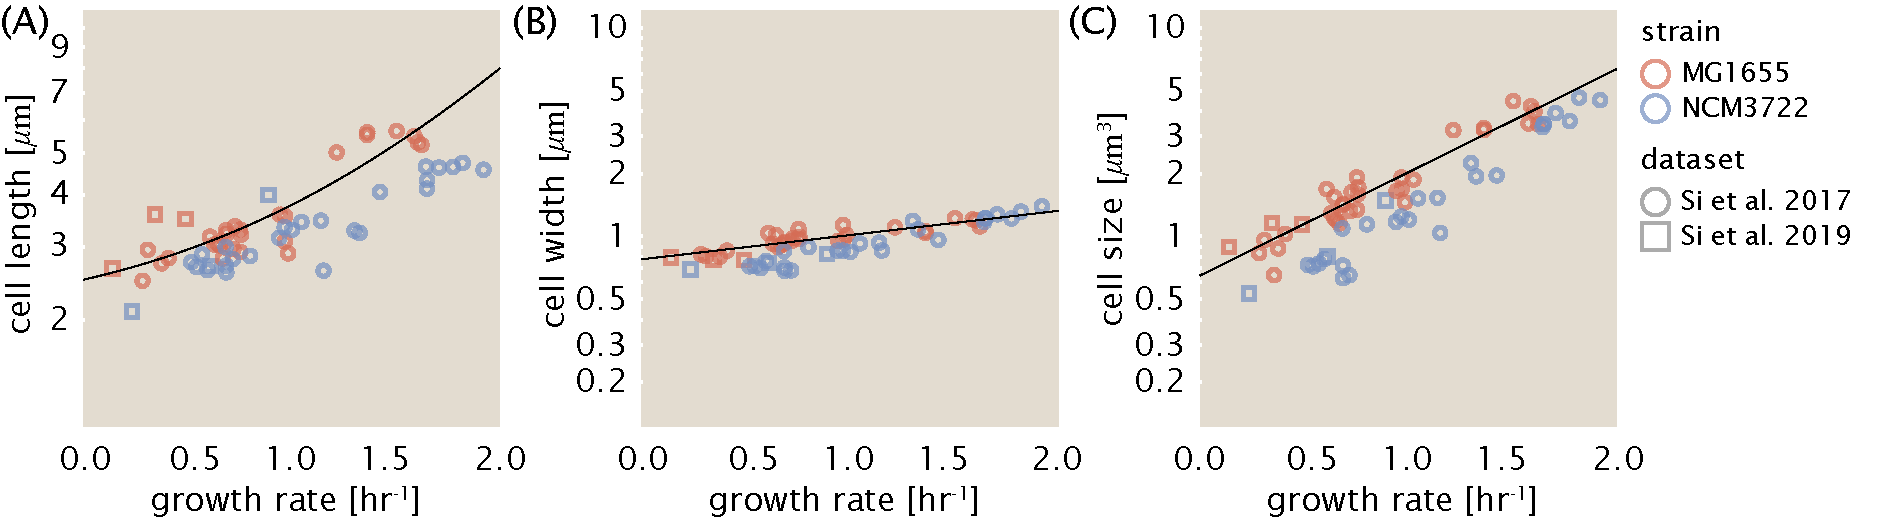
\includegraphics[width=1.0\textwidth]{SI_figs/final_cell_size_Si.pdf}
  \caption{\textbf{Summary of size measurements from Si \textit{et al.} 2017, 2019.}
	 	 Cell lengths and widths were measured from cell contours obtained from
	 	 phase contrast images, and refer to the long and short axis respectively.
	 	 (A) Cell lengths and (B) cell widths show the mean measurements reported
	 	 (they report 140-300 images and 5,000-30,000 for each set of samples;
	 	 which likely means about 1,000-5,000 measurements per mean value reported
	 	 here since they considered about 6 conditions at a time). Fits were made
	 	 to the  MG1655 strain data; length: 0.5 $e^{1.09 \cdot \lambda}$ + 1.76
	 	 $\mu$ m, width:  0.64 $e^{0.24 \cdot \lambda}$ $\mu$ m. (C) Cell size,
	 	 $V$, was calculated as cylinders with two hemispherical ends ($V$ = $\pi$
	 	 r$^2 \cdot$ ($l$ - $2r/3$)) where $r$ is half the cell width, and $l$ is
	 	 the cell length. The MG1655 strain data gave a best fit of 0.533 $e^{1.037
	 	 \cdot \lambda}$ $\mu$ m$^3$.}
  \label{fig:final_size_data_Si}
\end{figure}
